%%%%%%%%%%%%%%%%%%%%%%%%%%%%%%%%%%%%%%%%%%%%%%%%%%%%%%%%%%%%%%%%
\section{Validation Scenarios}
\label{sec:case_study_scenarios}

This section evaluates the controlled-pendulum case study in three scenarios.
Each scenario uses the references and metrics defined in Section~\ref{sec:case_study_reference_metrics}.
The baseline scenario verifies the FMU-only closed-loop co-simulation against the monolithic OpenModelica reference.
The contact scenario evaluates the integrated workflow with hybrid events, PID reset, and runtime plant-model switching.
The performance scenario benchmarks the computational benefit of activating the FEM model only near contact.

%%%%%%%%%%%%%%%%%%%%%%%%%%%%%%%%%%%%%%%%%%%%
\subsection{Baseline Closed Loop Without Contact}
\label{sec:case_study_baseline}

The baseline scenario is the numerical-verification case for the FMU-only closed loop without contact.
The system contains the setpoint generator, PID controller, dynamic drive, and FMU pendulum plant.
Sensor sampling and quantization are disabled.
This isolates the numerical effect of co-simulation coupling and of the macro communication step size.

The monolithic reference is the OpenModelica model \texttt{NoContact.Baseline}.
The primary comparison variable is the pendulum angle \(\theta\), because it is the closed-loop plant output.
The comparison uses \(E_{\infty,\theta}\) and \(E_{2,\theta}\) as defined in Section~\ref{sec:case_study_reference_metrics}.
The co-simulation is repeated for
\(\Delta t \in \{0.02, 0.01, 0.005, 0.001\}\,\mathrm{s}\).
The expected behavior is a decreasing trajectory error as the macro step size is refined.

\begin{figure}[t]
    \centering
    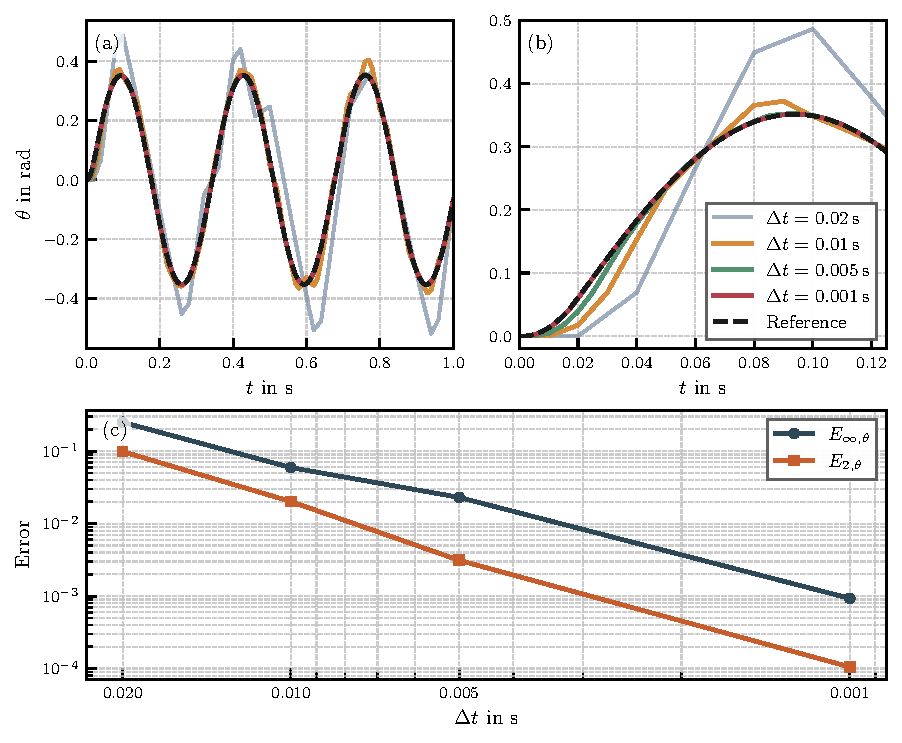
\includegraphics[width=\linewidth]{figures/6_case_study/controlled_pendulum/validation/baseline_step_convergence.pdf}
    \caption{Baseline closed-loop co-simulation without contact.
    Panel~(a) compares the full angle trajectory for different macro step sizes with the monolithic OpenModelica reference.
    Panel~(b) magnifies the first \(0.4\,\mathrm{s}\), where the coarse macro step produces the largest visible deviation.
    Panel~(c) reports the sampled angle errors \(E_{\infty,\theta}\) and \(E_{2,\theta}\) against the interpolated reference solution.
    The horizontal axis in panel~(c) is inverted so that macro-step refinement proceeds from left to right.}
    \label{fig:case_baseline_convergence}
\end{figure}

Figure~\ref{fig:case_baseline_convergence} shows the expected refinement behavior.
For \(\Delta t=0.02\,\mathrm{s}\), the angle trajectory visibly deviates from the reference during the first rise and the deviation grows over the full horizon.
For \(\Delta t=0.01\,\mathrm{s}\) and smaller, the trajectory follows the reference much more closely.
The zoomed panel confirms that the remaining differences decrease with the communication step size.

The error plot confirms the visual interpretation.
Both \(E_{\infty,\theta}\) and \(E_{2,\theta}\) decrease monotonically over the tested step sizes.
This verifies numerical convergence of the FMU-only closed-loop co-simulation toward the monolithic OpenModelica reference.

%%%%%%%%%%%%%%%%%%%%%%%%%%%%%%%%%%%%%%%%%%%%
\subsection{Multi-Model Switching With FEM Contact}
\label{sec:case_study_multimodel_contact}

The second scenario evaluates the integrated contact workflow.
The closed-loop system from Section~\ref{sec:case_study_controlled_pendulum_system} is reused without modification.
The plant is represented by the \texttt{MasterPendulum}.
It exposes the shared plant interface and selects internally between the FMU rigid-body model away from contact, the OpenSim model in an intermediate region, and the FEM model close to the wall.
The contact event drives two event connections.
One event reverses the angular velocity of the active internal model.
The other event resets the PID integrator.

The monolithic reference is the OpenModelica model \texttt{Contact.RigidContact} with integrator reset enabled.
The reference uses an ideal rigid impact law.
The \syssimx{} configuration uses a stiff compliant FEM contact formulation during contact-relevant phases.
The comparison is therefore a numerical verification against a rigid-contact reference and a workflow validation of the heterogeneous switched co-simulation.
It is not a physical validation of the FEM contact law.

The simulation horizon is \(t_{\mathrm{end}}=0.4\,\mathrm{s}\), and the macro communication step size is \(\Delta t=10^{-3}\,\mathrm{s}\).
The FEM pendulum uses Young's modulus \(E=2.1\cdot 10^{11}\,\mathrm{Pa}\), Poisson ratio \(\nu=0.3\), and density \(\rho=7850\,\mathrm{kg\,m^{-3}}\).
The normal contact stiffness is \(k_n=2\cdot 10^9\,\mathrm{N\,m^{-1}}\).
The \texttt{MasterPendulum} starts in FMU mode and uses a dwell time of \(0.01\,\mathrm{s}\) for switching hysteresis.

The primary comparison variables are the exposed angle \(\theta\) and the contact-event times.
The angle error is reported over the full horizon and over the contact window \(t\in[0.15,0.35]\,\mathrm{s}\).
The event-time error is computed from the five paired contact events of the co-simulation and the rigid-contact reference.

\begin{figure}[tbp]
    \centering
    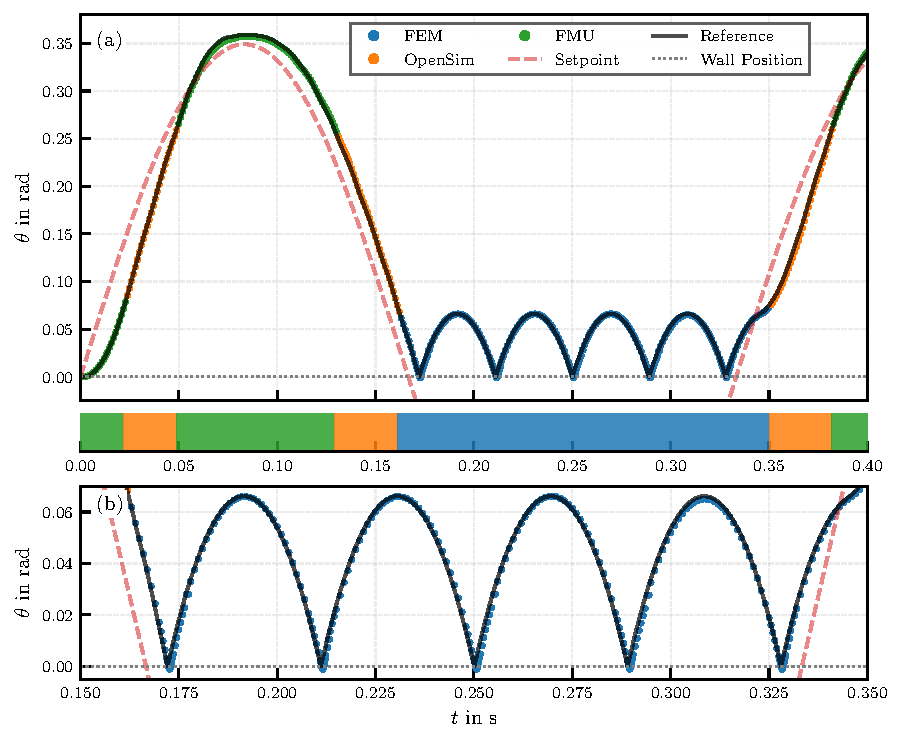
\includegraphics[width=\linewidth]{figures/6_case_study/controlled_pendulum/validation/multi_model_switching.pdf}
    \caption{Multi-model contact scenario with runtime plant-model switching.
    Panel~(a) shows the switched pendulum trajectory against the monolithic OpenModelica rigid-contact reference, with the active internal plant model indicated by the mode strip below the axes.
    Panel~(b) magnifies the contact window, where the FEM model is active and resolves the stiff compliant contact.
    The remaining deviations from the reference occur mainly during contact because the co-simulation uses a compliant FEM contact law, whereas the reference uses an ideal rigid impact model.}
    \label{fig:case_multimodel_contact}
\end{figure}

Figure~\ref{fig:case_multimodel_contact} shows that the switched trajectory follows the rigid-contact reference closely during free motion.
The largest deviations occur during the repeated rebounds at the wall.
This behavior is expected because the reference applies an ideal velocity reflection, while the co-simulation resolves contact through a stiff compliant FEM model.

The mode strip records seven accepted mode switches.
The early FMU\(\rightarrow\)FEM\(\rightarrow\)OpenSim\(\rightarrow\)FMU sequence is the start-up transient of the dwell-limited switching logic.
During the contact-relevant interval, the FEM model remains active and resolves all five wall contacts.

\begin{table}[tbp]
    \centering
    \small
    \caption{Trajectory and event-time errors for the multi-model contact scenario, computed against the interpolated OpenModelica rigid-contact reference.}
    \label{tab:case_multimodel_metrics}
    \begin{tabular}{llrr}
        \toprule
        \textbf{Quantity} & \textbf{Interval} & \(\boldsymbol{E_\infty}\) & \(\boldsymbol{E_2}\) \\
        \midrule
        \(\theta\) (rad)   & full horizon                     & \(5.244\cdot 10^{-3}\) & \(1.884\cdot 10^{-3}\) \\
        \(\theta\) (rad)   & contact window \([0.15,0.35]\,\mathrm{s}\) & --- & \(1.460\cdot 10^{-3}\) \\
        \(t_e\) (s)        & 5 paired contact events          & \(3.494\cdot 10^{-4}\) & --- \\
        \bottomrule
    \end{tabular}
\end{table}

Table~\ref{tab:case_multimodel_metrics} quantifies the trajectory and event-time deviations.
The maximum angle error is \(5.244\cdot 10^{-3}\,\mathrm{rad}\), which corresponds to approximately \(0.30^\circ\).
This maximum occurs inside the contact window.
The contact-window row therefore reports only \(E_{2,\theta}\), since the corresponding \(E_{\infty,\theta}\) is identical to the full-horizon value.

All five contact events of the reference are reproduced.
The largest event-time error is \(3.5\cdot 10^{-4}\,\mathrm{s}\), which is below one half of the macro communication step.
The PID reset event connection fires on each contact event.
This confirms that contact detection, event routing, plant-state update, and controller reset are exercised in one closed-loop run.

The switching consistency is evaluated from the \texttt{sync\_events} log of the \texttt{MasterPendulum}.
Across the seven accepted switches, the maximum state jump is \(3.47\cdot 10^{-18}\,\mathrm{rad}\) for \(\theta\) and \(7.11\cdot 10^{-15}\,\mathrm{rad\,s^{-1}}\) for \(\omega\).
These values are at numerical round-off level.
The state transfer between internal plant models therefore does not introduce visible discontinuities in the exposed plant trajectory.

This scenario verifies the integrated workflow rather than the isolated hybrid algorithm.
The isolated event-detection and event-handling mechanisms were verified in Section~\ref{sec:impl_hybrid_verification}.
The result here shows that heterogeneous pendulum models, hybrid contact events, runtime model switching, and PID reset can be combined in one closed-loop co-simulation.

%%%%%%%%%%%%%%%%%%%%%%%%%%%%%%%%%%%%%%%%%%%%
\subsection{Runtime Performance of Switched FEM Usage}
\label{sec:case_study_performance}

The third scenario benchmarks the computational benefit of runtime fidelity switching.
It uses the same contact mechanics as Section~\ref{sec:case_study_multimodel_contact}.
One configuration keeps the FEM pendulum active over the full trajectory.
The second configuration uses the \texttt{MasterPendulum} and activates the FEM model only near the wall.
Both configurations use the same macro communication step, FEM internal step, material parameters, contact stiffness, and input trajectory.
The simulation horizon is \(t_{\mathrm{end}}=0.4\,\mathrm{s}\).
The macro communication step and the FEM internal step are both \(10^{-3}\,\mathrm{s}\).
The contact stiffness is \(k_n=2\cdot 10^9\,\mathrm{N\,m^{-1}}\).
The switched configuration uses the position threshold \(0.075\,\mathrm{rad}\) for FEM activation and a dwell time of \(0.05\,\mathrm{s}\).

The full-FEM configuration is used as the high-fidelity benchmark for this comparison.
The switched contact workflow was already evaluated against the monolithic OpenModelica reference in Section~\ref{sec:case_study_multimodel_contact}.
This scenario therefore reports a benchmark of computational cost.
It does not establish correctness on its own.

\begin{figure}[tbp]
    \centering
    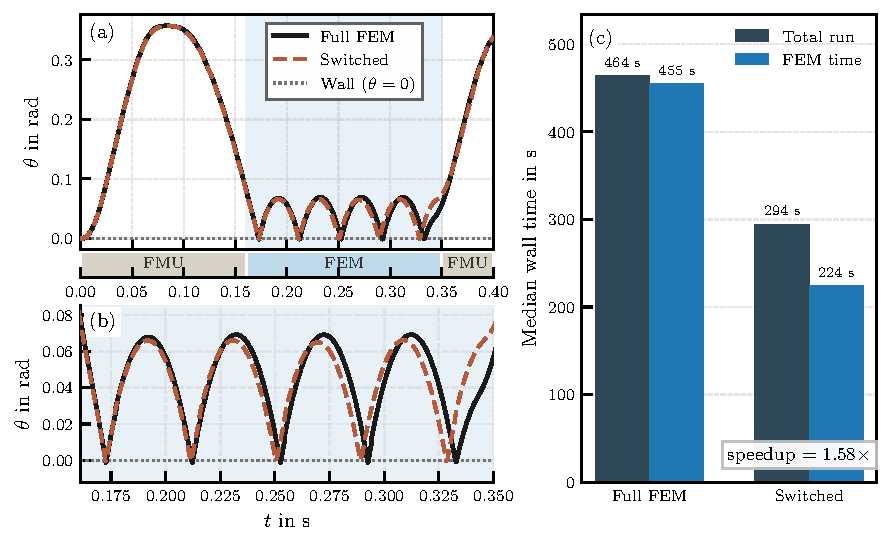
\includegraphics[width=\linewidth]{figures/6_case_study/controlled_pendulum/validation/performance_switching.pdf}
    \caption{Performance benchmark of full-FEM versus switched FEM execution.
    Panel~(a) compares the full-horizon angle trajectory of the full-FEM pendulum and the switched \texttt{MasterPendulum}.
    The mode strip below panel~(a) indicates when the switched run uses the FMU and FEM pendulum models.
    Panel~(b) magnifies the contact window, where the trajectory differences are concentrated.
    Panel~(c) reports the median total wall time and the median time spent in the FEM solver.
    The FEM time is a subset of the total run time.
    The medians are computed from five measured runs after one warm-up run.}
    \label{fig:case_performance_switching}
\end{figure}

Figure~\ref{fig:case_performance_switching} shows the trajectory and timing comparison.
The mode strip shows that the switched configuration enters FEM mode shortly before the first wall contact.
It remains in FEM mode throughout the repeated bounce sequence and returns to FMU mode afterwards.
The two trajectories agree closely outside the contact window.
The visible differences are concentrated during the rebounds.

\begin{table}[tbp]
    \centering
    \small
    \caption{Runtime and trajectory metrics for the performance benchmark over \(t_{\mathrm{end}}=0.4\,\mathrm{s}\).
    Wall times are reported as medians over repeated runs after excluding warm-up runs.}
    \label{tab:case_performance_metrics}
    \begin{tabular}{p{4.8cm} p{3.1cm} p{3.1cm} p{2.4cm}}
        \toprule
        \textbf{Metric} & \textbf{Full FEM} & \textbf{Switched} & \textbf{Relation} \\
        \midrule
        Total wall time
          & \(464.0\,\mathrm{s}\)
          & \(294.3\,\mathrm{s}\)
          & \(1.58\times\) speedup \\
        FEM solver wall time
          & \(455.0\,\mathrm{s}\)
          & \(224.3\,\mathrm{s}\)
          & \(2.03\times\) reduction \\
        FEM solver invocations
          & \(850\)
          & \(425\)
          & \(2.00\times\) reduction \\
        FEM-active simulated time
          & \(0.400\,\mathrm{s}\)
          & \(0.189\,\mathrm{s}\)
          & \(47.3\,\%\) of full \\
        Mode switches
          & \(0\)
          & \(2\)
          & --- \\
        \(E_{\infty,\theta}\) against full FEM
          & ---
          & \(2.839\cdot 10^{-2}\,\mathrm{rad}\)
          & --- \\
        \(E_{2,\theta}\) against full FEM
          & ---
          & \(8.202\cdot 10^{-3}\,\mathrm{rad}\)
          & --- \\
        \bottomrule
    \end{tabular}
\end{table}

Table~\ref{tab:case_performance_metrics} summarizes the runtime and trajectory metrics.
The switched configuration reduces the median total wall time from \(464.0\,\mathrm{s}\) to \(294.3\,\mathrm{s}\).
This corresponds to an end-to-end speedup of \(1.58\times\).
The FEM solver wall time decreases from \(455.0\,\mathrm{s}\) to \(224.3\,\mathrm{s}\), which corresponds to a reduction by \(2.03\times\).
This reduction is consistent with the smaller number of FEM solver invocations and with the reduced FEM-active simulated time.
The switched trajectory differs from the full-FEM benchmark by \(E_{\infty,\theta}=2.839\cdot 10^{-2}\,\mathrm{rad}\) over the full horizon.
This value reports the numerical cost of switching relative to the full-FEM benchmark.

The benchmark shows whether runtime fidelity switching reduces computational cost for the controlled-pendulum case study.
The expected benefit is obtained by avoiding FEM execution during phases where the high-fidelity contact representation is not needed.
The expected cost is a contact-window deviation relative to the full-FEM benchmark.
This accuracy and runtime tradeoff is discussed in Section~\ref{sec:case_study_discussion}.
